\documentclass[man,floatsintext,letterpaper,12pt]{apa7}

\usepackage[T1]{fontenc}
\usepackage[utf8]{inputenc}
\raggedbottom

\usepackage{csquotes}
\MakeOuterQuote{"}

\usepackage{booktabs}
\usepackage{caption}
\usepackage{setspace}
\captionsetup[figure]{font=doublespacing,justification=justified}
\captionsetup[table]{font=doublespacing}

\usepackage{hyperref}
\hypersetup{hidelinks,colorlinks=false}
\urlstyle{same}
\usepackage{lineno}
\linenumbers

\usepackage{amsmath}
\usepackage{amsfonts}
\usepackage{amssymb}

\usepackage[
  autocite=inline,
  style=apa,
  sortcites=true,
  sorting=nyt,
  backend=biber
  ]{biblatex}
  \addbibresource{../references.bib}
  \addbibresource{../r-references.bib}
  \addbibresource{../meta-references.bib}

\DeclareBibliographyCategory{asterisk}
\renewbibmacro*{begentry}{%
    \ifcategory{asterisk}%
    {*}%
    {}%
}
\newcommand*{\nocitemeta}[1]{%
    \nocite{#1}%
    \addtocategory{asterisk}{#1}%
}

\renewcommand{\postnotedelim}{\space}

\usepackage{comment}

\title{Reporting Bias, not External Focus: A Robust Bayesian Meta-Analysis and Systematic Review of the Attentional Focus Literature}
\shorttitle{Reporting bias, not external focus}

\renewcommand\author[1]{}
\renewcommand\affiliation[1]{}
\authorsnames[1, 2, 3, 4, 5, 5, 1, 1]{Brad McKay, Abbey E. Corson, Jeswende Seedu, Celeste S. De Faveri, Hibaa Hasan, Kristen Arnold, Faith C. Adams, Michael J. Carter\vspace{2ex}}
\authorsaffiliations{{Department of Kinesiology, McMaster University}, {School of Human Kinetics, University of Ottawa}, {Faculty of Health Sciences, McMaster University}, {School of Biomedical Sciences, McGill University}, {School of Interdisciplinary Science, McMaster University}}

\abstract{Evidence has ostensibly been accumulating over the past two decades suggesting that an external focus on the intended movement effect (e.g., on the golf club during a swing) is superior to an internal focus on body movements (e.g., on your arms during a swing) for skill acquisition. Seven previous meta-studies have all reported evidence of external focus superiority. The most comprehensive of these concluded an external focus enhances motor skill retention, transfer, and performance, leads to reduced eletromyographic activity during performance, and that more distal external foci are superior to proximal external foci for performance. Here, we re-analyzed these data using robust Bayesian meta-analyses that included several plausible models of publication bias. We found moderate to strong evidence of publication bias for all analyses. After correcting for publication bias, estimated mean effects were negligible: \emph{g} = 0.01 (performance), \emph{g} = 0.15 (retention), \emph{g} = 0.09 (transfer), \emph{g} = 0.06 (electromyography), and \emph{g} = -0.01 (distance effect). Bayes factors indicated data favored the null for each analysis, ranging from BF\textsubscript{01} = 1.3 (retention) to 5.75 (performance). We found clear evidence of heterogeneity in each analysis, suggesting the impact of attentional focus depends on yet unknown contextual factors. Our results contradict the existing consensus that an external focus is always more effective than an internal focus. Instead, focus of attention appears to have a variety of effects that we cannot account for, and on average those effects are small to nil. These results parallel previous metascience suggesting publication bias has obfuscated the motor learning literature.}

\keywords{Motor learning, Motor skills, Attentional focus, OPTIMAL theory, Skill acquisition, Metascience

\clearpage

\noindent \textbf{\emph{Public Significance Statement}}
\noindent A robust Bayesian meta-analysis showed that directing learners to focus their attention on their intended movement effects---often called an external focus---may have little-to-no effect on motor performance and learning on average. Although the consensus among researchers and practitioners has been that an external focus is superior to focusing on one's own body during practice, the present results suggest this may depend on unknown factors and our current understanding has been distorted by publication bias. These results highlight that a more cautious approach is necessary when recommending the use of external foci in applied settings until a more reliable body of literature can be established using preregistration, Registered Reports, and well-powered designs through multi-site collaborations.
}

\authornote{
\addORCIDlink{\hspace{-0.75ex}Brad McKay}{0000-0002-7408-2323}

\addORCIDlink{Michael J. Carter}{0000-0002-0675-4271}

Correspondence concerning this article should be addressed to Michael J. Carter, Department of Kinesiology, McMaster University. 1280 Main Street West, Hamilton, ON, Canada. L8S 4K1. Email: cartem11@mcmaster.ca; motorlab@mcmaster.ca
}

\begin{document}
\maketitle

Where should you focus when performing and/or learning a motor skill? The most basic of questions for a novice learner and an experienced performer alike. Is it better to focus on what you are doing: where your body is in space and how it is behaving? Or is it better to focus on what you intend to do: the end effect you are trying to achieve independent of how your body achieves it? This question has been the topic of decades of research comparing an internal focus of attention (i.e., focusing on your own body) to an external focus of attention (i.e., focusing on the intended effect of the action). Gabriele Wulf pioneered this area of inquiry in 1998, publishing a two-experiment article illustrating the benefits of adopting an external focus \autocite{wulf1998-meta}. In the experiments, instructing learners to focus on the wheels of a ski simulator (Experiment 1) or the markers on a balance platform (Experiment 2) led to improved motor learning compared to focusing on one's feet. Dozens of studies have since replicated these initial findings \autocites[see][for reviews]{wulf2007,wulf2013}.

Previous reviews have argued that research shows benefits of an external focus in four main areas: (a) effectiveness at accuracy and balance tasks, (b) efficiency in electromyographic activity, force production, speed, and endurance tasks, (c) promoting automaticity, and (d) enhancing movement form \autocite{chua2021,wulf2016,wulf2013,wulf2007}. A leading explanation for the mechanism causing these benefits is goal-action coupling: a process proposed in Wulf and Lewthwaite's (\citeyear{wulf2016}) OPTIMAL theory involving a shift at the neural level that simultaneously directs action toward success and stifles deleterious self-focused cognition. Although focus of attention is fundamental to the OPTIMAL theory, various perspectives in motor behavior have offered complementary accounts for external focus benefits. For example, it has been argued from the constraints-based approach that an external focus promotes the search of the task during practice and provides a constraint on emerging actions \autocite{davids2003}. It has also been argued that actions and perceptions share a common (cognitive) code; therefore, focusing on the intended (perceptual) effect of an action is consistent with its underlying neural coding \autocite{wulf2001,prinz1990,hommel2001}. While research continues to explore the putative mechanisms, there is consensus in the motor learning community that adopting an external focus of attention can improve motor performance, retention, transfer, and movement efficiency---at least most of the time \autocite{lee2021a,chua2021,makaruk2020,kim2017,li2022,grgic2021,grgic2022,nicklas2022}.\footnotemark{}

\footnotetext{Despite acknowledging this as the general consensus in the field, it is important to note that there are mixed findings and alternative discussions in this area of research \autocite[e.g.,][]{bernier2016,perkins2003-meta,maurer2013-meta,collins2016,brick2014,peh2011,lawrence2011-meta,zentgraf2009-meta,emanuel2008-meta,canning2005,schorer2012}.}

Buttressed by the largely positive results in the research literature, external focus of attention is now widely recommended outside of academia, including by sport coaches \autocites[skating:][]{smale2021}[golf:][]{neumann2017}[tennis:][]{kuzdub2022}[baseball:][]{peterson2019}, fitness coaches \autocite{winkelman2015,kompf2015}, and therapists \autocite{magne2017,lo2019}. Researchers continue to study the use of externally focused instructions and feedback in clinical settings \autocite{johnson2023} and are currently developing strategies for increasing awareness of the research among rehabilitation professionals \autocite{hussien2023a,hussien2023b,hussien2023}. As external focus becomes evermore mainstream, recent concerns that much of the motor learning literature may be exaggerated by reporting bias \autocite[e.g.,][]{lohse2016,mckay2022b,mckay2022a,twomey2021b,mesquida2022} underlines the need for careful assessment of the evidence. The external focus literature may be especially at risk because substantial reporting bias has been found in the motor learning literature investigating the other factors within OPTIMAL theory \autocite{mckay2022b,bacelar2022b,mckay2023}. Note that reporting bias encompasses various forms of selection bias that limit the availability of data. Potential reporting bias mechanisms can be modeled, though models cannot determine the specific reason for censorship within a literature.

\subsection{Previous Meta-Analyses}

There have been seven meta-analyses comparing the effects of internal and external focus instructions on motor outcomes. Five have focused on specific task-types: balance \autocite{kim2017}, jumping \autocite{makaruk2020}, sprinting \autocite{li2022}, strength \autocite{grgic2021}, and endurance \autocite{grgic2022}. A sixth included all motor tasks and focused specifically on the immediate effect on performance \autocite{nicklas2022}. Chua and colleagues (\citeyear{chua2021}) conducted the most comprehensive meta-analysis of the seven, including all task-types and estimating effects on performance, retention, transfer, electromyography activity, and the distance effect. All seven studies reported the results of random effects meta-analyses as the primary estimates for the effect of focus of attention. Although there was some variance in point estimates and confidence intervals, each of the studies reported evidence that an external focus is superior to an internal focus.

Importantly, a random effects model assumes no reporting bias and has been shown to be quite biased in the presence of selective reporting for statistical significance \autocite{bartos2023a,bom2019,carter2015,carter2019,kvarven2020,stanley2017,stanley2022}. Two of the seven previous studies \autocite{chua2021,kim2017} reported evidence of funnel plot asymmetry, which is consistent with selective reporting of significant results. Two studies did not find evidence of funnel plot asymmetry \autocite{nicklas2022,li2022}, and the other three did not investigate reporting bias at all \autocite{grgic2021,grgic2022,makaruk2020}. Both studies that observed evidence of reporting bias conducted a fail-safe-style sensitivity analysis, but did not correct the primary estimates for the presence of bias. The meta-analysis by \textcite{chua2021} did calculate worst-case-scenario estimates based on a random effects meta-analysis of the non-significant results. Thus, although reporting bias may be prevalent in the field of motor learning \autocite{lohse2016}, and two previous meta-analyses have found evidence of reporting bias in the attentional focus literature \autocite{chua2021,kim2017}, the primary estimates from all previous meta-analyses assume bias is absent.

Consistent with the other studies, \textcite{chua2021} reported moderate benefits of an external focus for learning measures (\emph{g} = 0.58) and small benefits for performance measures (\emph{g} = 0.26) and the distance effect (\emph{g} = 0.22). Chua and colleagues also reported a large effect on electromyography activity (\emph{g} = 0.83). In lieu of bias-corrected estimates, worst-case scenario estimates were calculated to evaluate how sensitive the primary estimates were to an assumed model of reporting bias. Under the assumed model, significant results in the predicted direction are published without censorship, and all non-significant results and significant results in the opposite direction are censored at the same rate. The worst-case scenario is simply the random effects estimate of all the non-preferred outcomes as a preference for significant results in the predicted direction cannot upwardly bias an estimate if significant results are removed. If the worst-case scenario is positive, then one can conclude that no amount of reporting bias could attenuate the point estimate to the null value. However, this conclusion is only merited if censorship is entirely captured by the assumed model. If other plausible mechanisms of censorship are present, then the assumed model does not hold, and the worst-case scenario estimates can no longer be considered as such.

Although \textcite{chua2021} concluded that no amount of reporting bias could attenuate the effect to the null value for any measure (performance, retention, transfer, electromyography, and the distance effect), there are several plausible censorship mechanisms that were unexplored. For example, it is plausible that nearly significant results, often called non-significant trends \autocite{otte2022}, were censored less than other non-significant trends. It is also possible that point estimates favoring an internal focus were the least preferred result. If these plausible alternative censorship mechanisms were active in the attentional focus literature, then the random effects estimate of "all non-significant in the predicted direction" results would be positively biased. Although \textcite{chua2021} concluded that external focus superiority is not sensitive to reporting bias, it remains unknown if that conclusion is sensitive to the form of reporting bias that was assumed.

\subsection{Present Study}

Seven previous meta-analyses provide primary estimates of the potential benefit of an external focus of attention while assuming reporting bias is absent. Given the evidence of reporting bias reported in two of those studies \autocite{chua2021,kim2017}, along with evidence of extensive bias in related literatures \autocite[e.g.,][]{lohse2016,mckay2023}, bias-corrected estimates are needed. There are several plausible mechanisms of reporting bias, and the true model is unknowable. Therefore, using a robust Bayesian approach to meta-analysis \autocite{bartos2023}, we leveraged Bayesian model-averaging to fit several plausible models of reporting bias to the attentional focus literature examined by \textcite{chua2021}. Greater weight was given to the models that best accounted for the results and less weight was given to poorly performing models. This approach allowed us to calculate reporting-bias-adjusted estimates for the effect of attentional focus on motor learning, performance, electromyography activity, and for the distance effect. Our approach naturally allowed us to evaluate Chua and colleagues' (\citeyear{chua2021}) claims that no amount of reporting bias could attenuate the effect to the null value.

In addition to censorship mechanisms, we also explored the role of \emph{post hoc} outcome selection leading to potentially exaggerated estimates. The previous seven meta-analyses either did not specify exactly how outcomes were selected for analysis \autocite{grgic2021,grgic2022,kim2017,makaruk2020,li2022}, excluded studies that had more than one performance measurement unless the measures could be ranked and a primary measure could be selected \autocite{nicklas2022}, or selected the outcome positioned as primary in the original research article \autocite{chua2021}. The external focus literature has not made use of preregistration or Registered Reports, so it is possible that the most impressive results have sometimes been positioned as primary because they were the most impressive. If this sort of \emph{post hoc} selection is present, then selecting outcomes based on their status in the original article may lead to biased estimates. To evaluate the possibility of \emph{post hoc} selection bias, we extracted effect size estimates for the retention test outcomes that were not selected by \textcite{chua2021}, but could have been, and compared them to the selected "primary" outcomes.

In the present study, we addressed the following questions: (a) What is the reporting-bias-adjusted estimate for the effect of attentional focus on learning, performance, electromyography activity, and the distance effect? (b) How sensitive are random effects estimates to the assumption that reporting bias is absent? (c) How sensitive are Chua and colleagues' (\citeyear{chua2021}) conclusions that no amount of reporting bias could attenuate the effect to the null value to the specific model of censorship that was evaluated? and (d) How influential was \emph{post hoc} selection bias on the estimated benefits of an external focus of attention on retention performance?

\section{Methods}

\subsection{Transparency and Openness}

We adhered to the Meta-Analysis Journal Reporting Standards (MARS) guidelines for meta-analytic reporting \autocite{appelbaum2018}. The data, code, and preregistration for this study are publicly available at \url{https://osf.io/vfmx2} \autocite{mckay-carter2024}.\footnotemark{} The data for each primary outcome measure were collected and reported by \textcite{chua2021}. Our re-analysis of those data was not preregistered as we were already aware of Chua and colleagues' (\citeyear{chua2021}) primary conclusions and had seen the data visualizations in their study. Data for up to three additional outcomes from each experiment that examined retention test performance were collected and analyzed according to our preregistered protocol. There were no deviations from our preregistration.
\footnotetext{Data and scripts are also available at \url{https://github.com/cartermaclab/proj_foa-optimal-theory}.}

Statistical analyses were conducted using
\texttt{R} \autocite[Version 4.3.2;][]{R-base} and the \texttt{R}-packages 
\emph{compute.es} \autocite[Version 0.2.5;][]{R-compute.es},
\emph{daff} \autocite[Version 0.3.5;][]{R-daff},
\emph{extrafont} \autocite[Version 0.19;][]{R-extrafont},
\emph{faux} \autocite[Version 1.2.1;][]{R-faux},
\emph{ggdist} \autocite[Version 3.2.1;][]{R-ggdist},
\emph{gt} \autocite[Version 0.9.0;][]{R-gt},
\emph{magick} \autocite[Version 2.7.4;][]{R-magick},
\emph{metafor} \autocite[Version 4.0.0;][]{R-metafor},
\emph{patchwork} \autocite[Version 1.2.2;][]{R-patchwork},
\emph{plotly} \autocite[Version 4.10.2;][]{R-plotly},
\emph{PublicationBias} \autocite[Version 2.3.0;][]{R-PublicationBias},
\emph{renv} \autocite[Version 0.17.2;][]{R-renv},
\emph{RoBMA} \autocite[Version 2.3.2;][]{R-RoBMA},
\emph{stringi} \autocite[Version 1.7.12;][]{R-stringi},
and \emph{tidyverse} \autocite[Version 2.0.0;][]{R-tidyverse} were used in this project.

\subsection{Eligibility}

Our analysis was restricted to the studies included in the study by \textcite{chua2021}, meaning our study inherits the inclusion criteria imposed in their study: (a) published in English between February 1998 and April 2019, (b) in a peer-reviewed journal, (c) compared internal and external foci of attention, or at least two types of external focus, (d) measured motor learning or performance, (e) used a within-participant design to measure performance and a between participants design to measure learning, (f) included sufficient data to calculate effect sizes, and (g) were experiments.

\subsection{Data Collection Process}

The data reported by \textcite{chua2021} were extracted directly from the published article. Additionally, up to three outcomes were extracted from each experiment included in the meta-analysis of retention test performance.\footnotemark{} Data were extracted in duplicate by a team of six researchers working independently (AC, JS, CDF, HH, KA, FA). The lead author evaluated each pair of extractions using the \texttt{R} package \texttt{daff} \autocite{R-daff} for consensus and resolved all conflicts.
\footnotetext{We chose to focus on retention effects because the performance estimates were already small. The retention estimates were substantial, and retention tests are often the focal learning measure in an experiment. Almost all transfer tests were from studies that also included a retention test, so focusing on retention outcomes was the simplest way to test our research question.}

Outcome measures were selected for extraction based on our preregistered priority list (see Table \ref{tab:table1}). A priority list achieved two goals. First, it prevented selection bias when several outcomes were reported in a study by establishing which outcomes to select \emph{a priori}. Second, the list prioritized outcomes most connected to the goal of the task over outcomes only correlated with success. This ensured the dependent variables most indicative of goal-action coupling were selected from each study.

\begin{table}[t]
    \caption{Priority list for extracting outcome measures.}
    \label{tab:table1}
    \small
    \begin{tabular}{@{}clcl@{}}
        \toprule
        Priority & Measure & Priority & Measure \\
        \midrule
        1 & Absolute error & 6 & Relative timing error \\
        2 & Root mean squared error / Total error & 7 & Absolute constant error \\
        3 & Accuracy points & 8 & Movement time \\
        4 & Variable error & 9 & Movement form (Expert raters) \\
        5 & Absolute timing error & 10 & Other \\
        \bottomrule
    \end{tabular}
\end{table}

The sample sizes, direction of effect, means, and standard deviations were extracted for each measure when available. If standard deviations were not reported, data were extracted in the following order of priority: means and standard errors, \emph{F}-values, then \emph{t}-values. If the required data were not reported in the text of the article, but were presented in figures with error bars, then the mean and standard deviation were extracted by digitizing the plots \autocite{rohatgi2022}. Data from six studies were digitized. If data could not be extracted with plot digitization, then the authors were emailed, and the data were requested. If the authors did not respond, a follow up email was sent. Emails were sent to authors requesting data for five effects, and one author responded with the requested data. Hedges' \emph{g} for the newly extracted outcomes was calculated using the \texttt{R} package \texttt{compute.es} \autocite{R-compute.es}. Risk of bias from methodological weaknesses was well probed by \textcite{chua2021} and was not revisited in this study.

\subsection{Synthesis Methods}

\subsubsection{Influential Cases}

We screened the data for influential cases using the \texttt{R} package \texttt{metafor} \autocite{viechtbauer2010a}. After fitting univariate random effects models for each meta-analysis, externally standardized residuals and Cook's distances were calculated. Studies identified as extreme by both measures were considered influential and a sensitivity analysis was conducted with the studies removed.\footnotemark{}
\footnotetext{Our approach to influential case screening differed from the approach employed by \textcite{chua2021} and we therefore arrived at a different number of outliers for each analysis (see Supplementary A for more details).}

\subsubsection{Reporting Bias}

We implemented a robust Bayesian approach \autocite{bartos2023} to reanalyze the five meta-analyses reported by \textcite{chua2021}. We used neutral default priors for the presence of an effect (Normal(M = 0, SD = 1), \emph{p} = 0.5), the presence of heterogeneity (InvGamma(1, 0.15), \emph{p} = 0.5), and the presence of reporting bias (\emph{p} = 0.5). Reporting bias was probed using selection models and funnel plot regression models. In the selection model class, six different weight-function models were fit to model censorship based on specific \emph{p}-value thresholds. For example, one selection model captures the possibility that significant results in the predicted direction are more likely to survive to be published than both null results and significant results in the unpredicted direction. Another selection model captures the possibility that results in the unpredicted direction are the least likely to survive censorship, while non-significant trends are more likely than other null results, but not as likely as significant results to survive.

A total of six selection models capturing different plausible censorship scenarios are assigned half of the prior probability that reporting bias exists. The other half of the prior probability is allocated to funnel plot regression models. The precision-effect test (PET) and precision-effect estimate with standard errors (PEESE) respectively model a linear and quadratic relationship between standard error and effect size. If the data were censored such that lower \emph{p}-values had a higher probability of surviving, a correlation would emerge between two otherwise independent causes of \emph{p}-values: effect sizes and standard errors. The PET method fits a linear relationship between effect size and standard error, modeling a consistent level of censorship across studies. The PEESE method fits a quadratic relationship, reflecting the possibility that studies with small standard errors, and thus large samples, are likely to be reported regardless of the results, and small studies with large standard errors require increasingly impressive results to garner publication.\footnotemark{}
\footnotetext{Priors for the six selection models were: $\omega$[two-sided: 0.05] $\sim$ CumDirichlet(1, 1), $\omega$[two-sided: 0.1, 0.05] $\sim$ CumDirichlet(1, 1, 1), $\omega$[one-sided: 0.05] $\sim$ CumDirichlet(1, 1), $\omega$[one-sided: 0.05, 0.025] $\sim$ CumDirichlet(1, 1, 1), $\omega$[one-sided: 0.5, 0.05] $\sim$ CumDirichlet(1, 1, 1), $\omega$[one-sided: 0.5, 0.05, 0.025] $\sim$ CumDirichlet(1, 1, 1, 1). Priors for the two regression models were: PET $\sim$ Cauchy(0, 1)[0, Inf], PEESE $\sim$ Cauchy(0, 5)[0, Inf].}

A total of 36 models were fit to the data with every combination of the eight reporting bias models, models assuming an effect, no effect, heterogeneity, no heterogeneity, and no reporting bias (see Supplementary B for more details). The estimates of each model were combined using Bayesian model-averaging, where model estimates are weighted based on how well the model fit the data. A single posterior distribution was generated for the average effect of an external focus and the average value of \emph{tau}---the estimated heterogeneity. Further, Bayes Factors were calculated measuring the evidence in favor of an effect, the presence of heterogeneity, and reporting bias.

\subsubsection{Post-Hoc Selection Bias}

A multi-level mixed effects model with outcomes nested in study, and with cluster-robust standard errors compared the outcomes selected by \textcite{chua2021} to the additional outcomes that might have been selected instead. Profile analysis was conducted to ensure the model converged on unique solutions for estimates of \emph{Mu} (the mean effect of external focus in the population) and \emph{tau}.

\section{Results}

Model-averaged posterior distributions for each analysis with and without outliers are presented in Figure \ref{fig:fig1}.\footnotemark{}
\footnotetext{Model convergence diagnostics were conducted for all RoBMA \autocite{R-RoBMA} analyses. In each case, Rhat convergence values were less than 1.05 and effect sampling sizes were a few hundred or more.}

\subsection{Performance}

Influence analyses revealed four studies \autocites[][]{marchant2009b-meta,nadzalan2015-meta,porter2010-meta}[][Experiments 1 and 2]{sherwood2014-meta} could be considered outliers in the performance meta-analysis. We report the results with all studies included first, then with outliers removed. The mean of the model-averaged posterior distribution for the difference between external and internal foci of attention on motor skill performance was \emph{g} = 0.01, 95\% credible interval: 0, 0.17. The data were over 5 times more compatible with the null hypothesis than the alternative, BF\textsubscript{10} = 0.17. There was clear evidence of heterogeneity, $\tau$ = 0.40, BF\textsubscript{rf} = Infinite. There was also clear evidence of publication bias, BF\textsubscript{pb} = 162,651.73. Removing influential cases did not substantively change the conclusions: \emph{g} = 0.02, 95\% credible interval: 0, 0.16, BF\textsubscript{10} = 0.26; $\tau$ = 0.25, BF\textsubscript{rf} = 602774614; BF\textsubscript{pb} = 97,268.05.

\clearpage

\begin{figure}[htbp]
    \caption{Posterior plots of the standardized mean difference with and without outliers.}
    \centering
    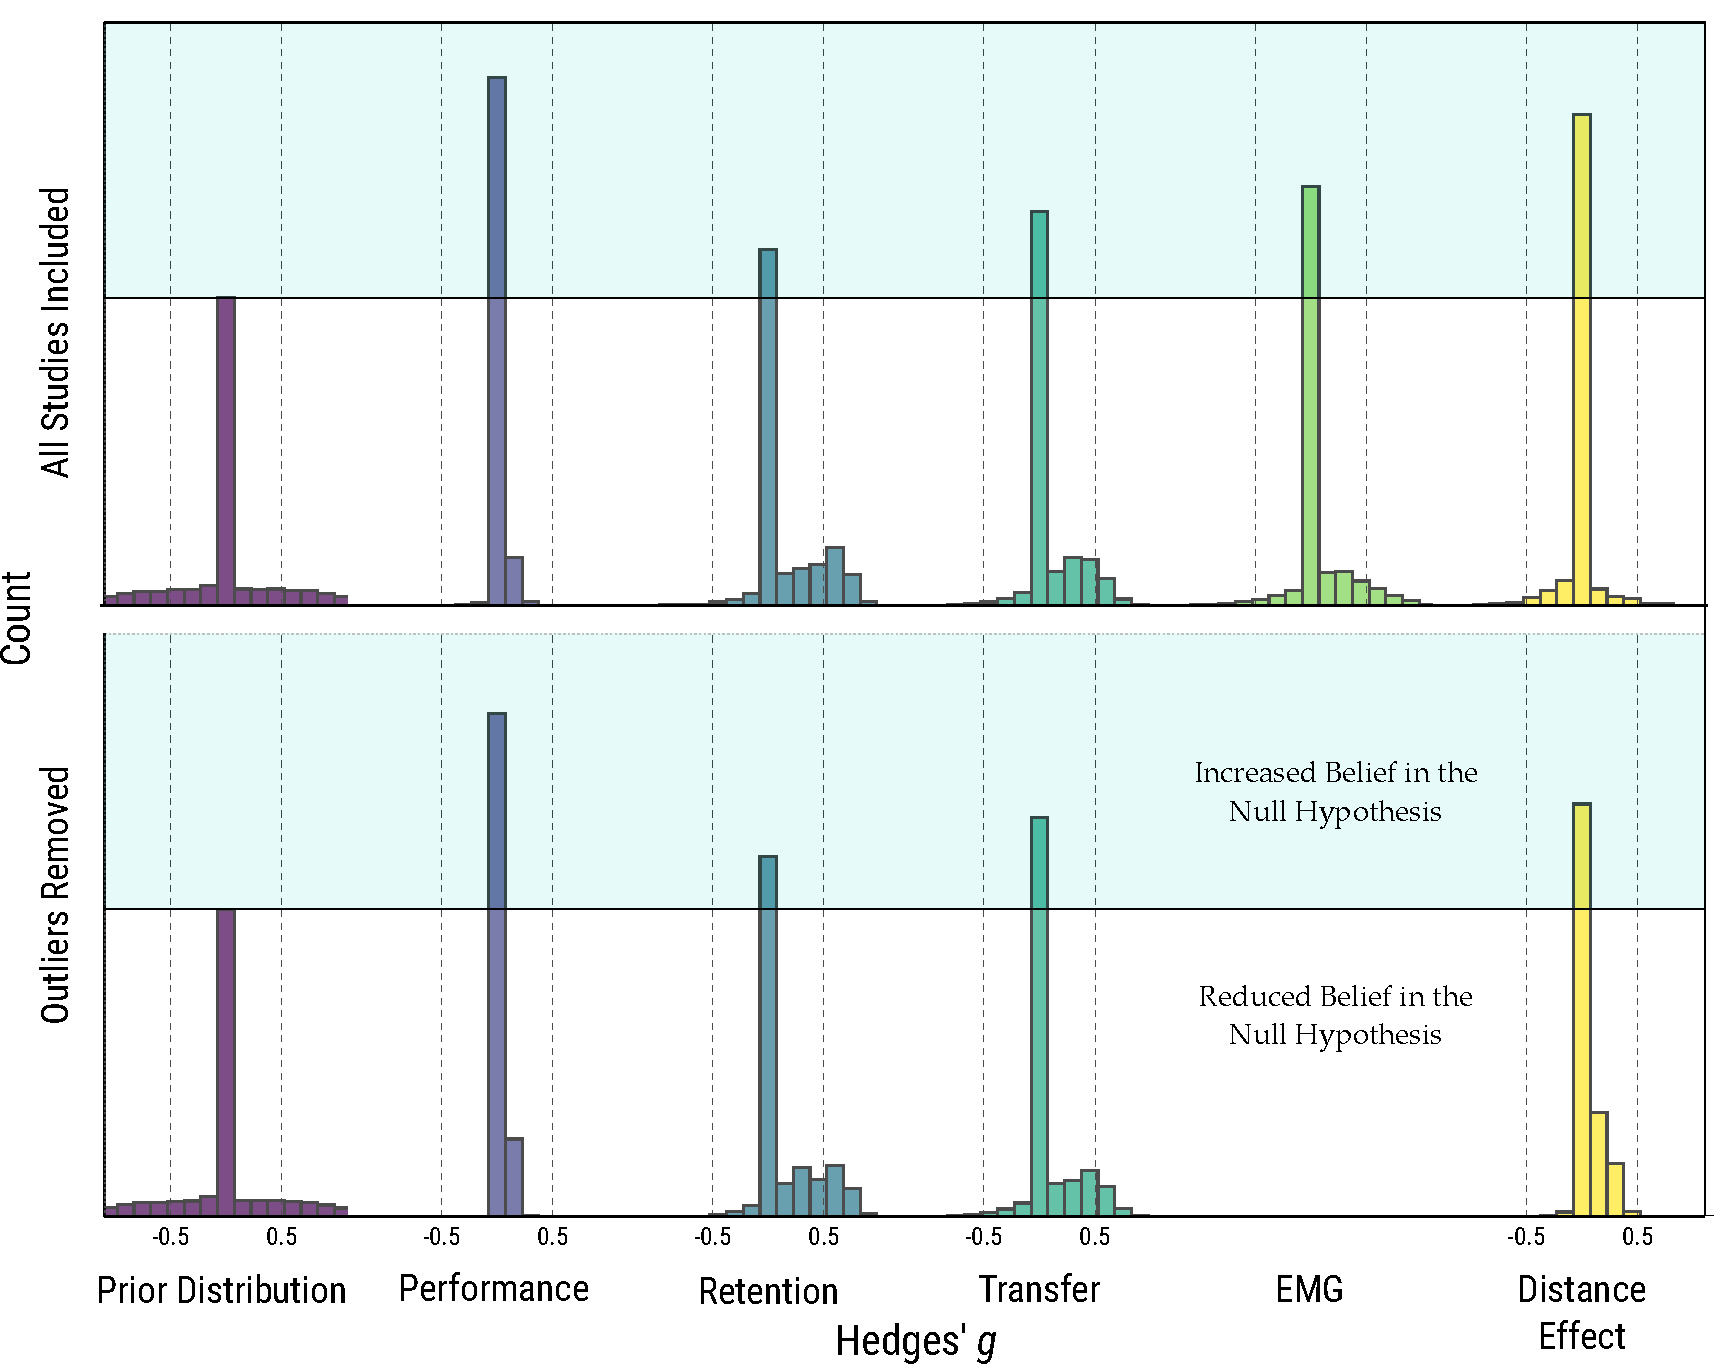
\includegraphics[scale=0.55]{../../figs/fig1.pdf}
    \setlength{\belowcaptionskip}{-2em}
    \caption*{\singlespacing \small Note. \normalfont The effect size estimates (\emph{g}) of each meta-analysis with all studies included (top row) and with outliers removed (bottom row). The histograms in the first column reflect the prior distribution, with 50\% of the probability density concentrated on zero effect (the null hypothesis) and 50\% of the density normally distributed (\emph{M} = 0, \emph{SD} = 1). The model-averaged posterior distributions for performance, retention, transfer, electromyography, and the distance effect are presented in the second through sixth columns, respectively. Increased belief in the null hypothesis is visible for each analysis, illustrated by the increased height of the spike at \emph{g} = 0 in all posteriors relative to the prior distribution.}
    \label{fig:fig1}
\end{figure}

\clearpage

\subsection{Retention}

Two studies \autocite{ahmad2013-meta,tse2019-meta} were identified as possible outliers in the retention test meta-analysis. Again, the results with all studies included are reported first, then with outliers removed. The mean of the model-averaged posterior distribution for the effect of focus of attention on retention was \emph{g} = 0.15, 95\% credible interval: -0.17, 0.74. The data were somewhat more consistent with the null hypothesis than the alternative, BF\textsubscript{10} = 0.75. There was clear evidence of heterogeneity, $\tau$ = 0.65, BF\textsubscript{rf} = Infinite. The data were 5.9 times more compatible with models assuming publication bias than without, BF\textsubscript{pb} = 5.92. Removing two influential cases did not substantively change the conclusions: \emph{g} = 0.14, 95\% credible interval: -0.18, 0.73, BF\textsubscript{10} = 0.73; $\tau$ = 0.50, BF\textsubscript{rf} = 1,688,117,430.52; BF\textsubscript{pb} = 7.62.

\subsection{Transfer}

One possible outlier \autocite{tse2019-meta} was identified in the transfer test meta-analysis. The mean of the model-averaged posterior distribution of all transfer outcomes was \emph{g} = 0.09, 95\% credible interval: -0.21, 0.62. The results were somewhat more likely under the null hypothesis than the alternative, BF\textsubscript{10} = 0.57. There was clear evidence of heterogeneity, $\tau$ = 0.56, BF\textsubscript{rf} = Infinite. The data were more than 6.4 times more likely under models assuming publication bias, BF\textsubscript{pb} = 6.45. Removing one influential case did not substantively change the conclusions: \emph{g} = 0.09, 95\% credible interval: -0.23, 0.63, BF\textsubscript{10} = 0.55; $\tau$ = 0.45, BF\textsubscript{rf} = 101,220.12; BF\textsubscript{pb} = 9.06.

\subsection{Electromyography}

There were no outliers identified in the electromyography meta-analysis. The mean of the model-averaged posterior distribution for the effect of attentional focus on electromyography activity was \emph{g} = 0.06, 95\% credible interval: -0.35, 0.69. The data were twice as likely under the null hypothesis as the alternative, BF\textsubscript{10} = 0.47. There was clear evidence of heterogeneity, $\tau$ = 0.49, BF\textsubscript{rf} = Infinite. There was very strong evidence of publication bias, BF\textsubscript{pb} = 26.40.

\subsection{Distance Effect}

One possible outlier \autocite{lohse2014-meta} was identified in the distance effect meta-analysis. The mean of the model-averaged posterior distribution for the difference between distal and proximal external foci was \emph{g} = -0.01, 95\% credible interval: -0.38, 0.30. The results were over 3.8 times more likely under the null hypothesis than the alternative, BF\textsubscript{10} = 0.26. There was clear evidence of heterogeneity, $\tau$ = 0.42, BF\textsubscript{rf} = 25.58. There was overwhelming evidence of publication bias, BF\textsubscript{pb} = 31.18. Removing the influential case did not substantively change the conclusions: \emph{g} = 0.06, 95\% credible interval: 0, 0.32, BF\textsubscript{10} = 0.52; $\tau$ = 0.42, BF\textsubscript{rf} = 2.38; BF\textsubscript{pb} = 2.97.

\subsection{Selection Moderator}

Outcomes selected for inclusion in Chua and colleagues' (2021) meta-analysis of retention performance were somewhat larger (\emph{g} = 0.74, 95\% confidence interval: 0.49, 0.99) than the additional outcomes that could have been extracted but were not (\emph{g} = 0.60, 95\% confidence interval: 0.27, 0.93; see Figure \ref{fig:fig2}). However, the difference between selected and not-selected outcomes was not statistically significant, \emph{F}(1, 45) = 1.62, \emph{p} = 0.21.

\clearpage

\begin{figure}[htbp]
    \caption{Forest plot of retention outcomes separated by "selected" moderator.}
    \centering
    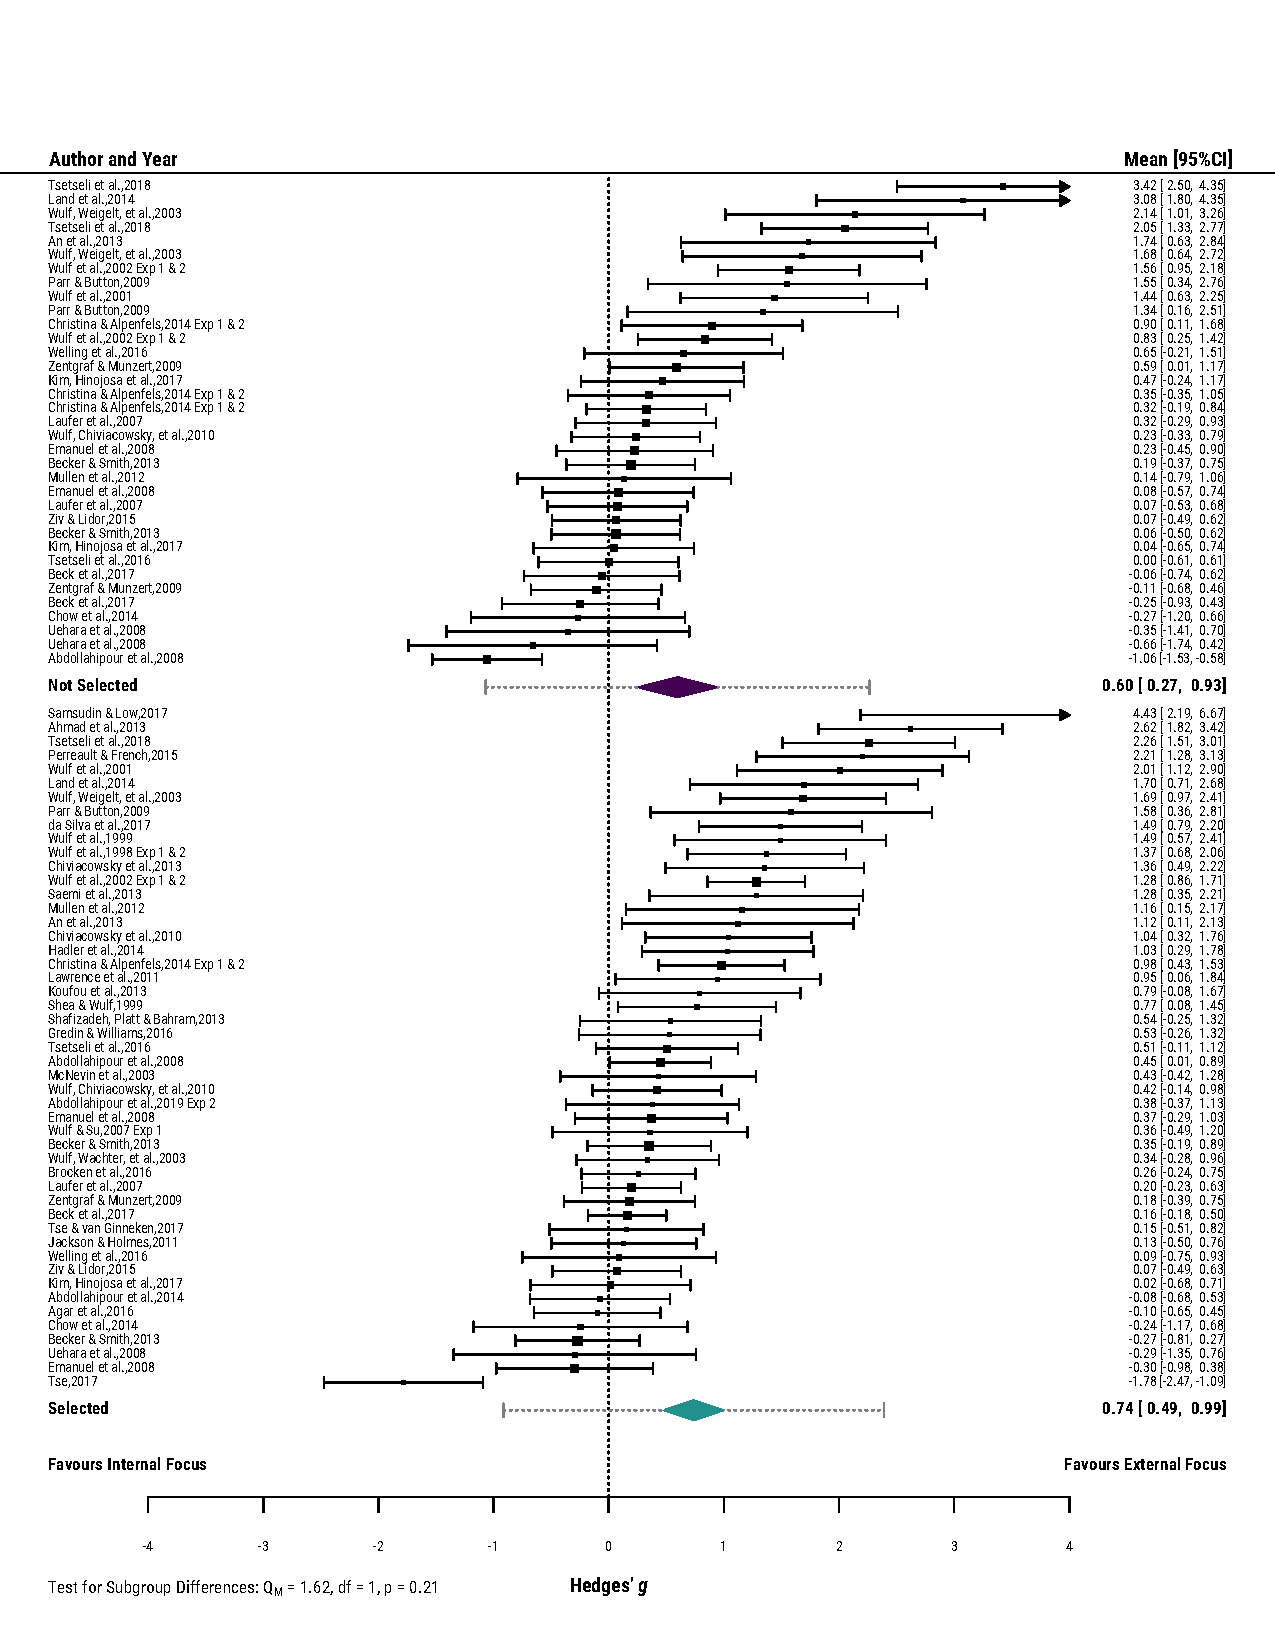
\includegraphics[scale=0.62]{../../figs/fig2.pdf}
    \setlength{\belowcaptionskip}{-2em}
    \caption*{\singlespacing \small Note. \normalfont Standardized mean difference (\emph{g}) and 95\% confidence intervals for each study included in the meta-analysis of retention outcomes. The green polygon represents the mean and 95\% confidence interval for outcomes that \textcite{chua2021} selected for analysis. The purple polygon represents the estimate for outcomes reported in the original experiments but were not selected by \textcite{chua2021}. The error bars extending from both polygons reflect the 95\% prediction interval, illustrating the range of outcomes we would expect to observe in 95\% of studies randomly sampled from the same population of studies included in this analysis. The prediction intervals account for the substantial unexplained heterogeneity present in these data, showing that even without correcting for publication bias we would expect outcomes across the entire plausible range of effects.}
    \label{fig:fig2}
\end{figure}

\clearpage

\subsection{Individual Model Fit}

As implied by the results of each analysis, the best performing models overall assumed heterogeneity, publication bias, and zero effect (see Figure \ref{fig:fig3}). The best fitting publication bias models were the PET and PEESE funnel plot regression models, as well as the selection models that assumed directional hypotheses, particularly those that modeled censorship based on the direction of the point estimate. This pattern of findings suggests complex, results-based selection mechanisms linked to more than just statistical significance.

\clearpage

\begin{figure}[htbp]
    \caption{Total Inclusion Bayes Factor for each model relative to the ensemble, summed across each of the five analyses with and without outliers.}
    \centering
    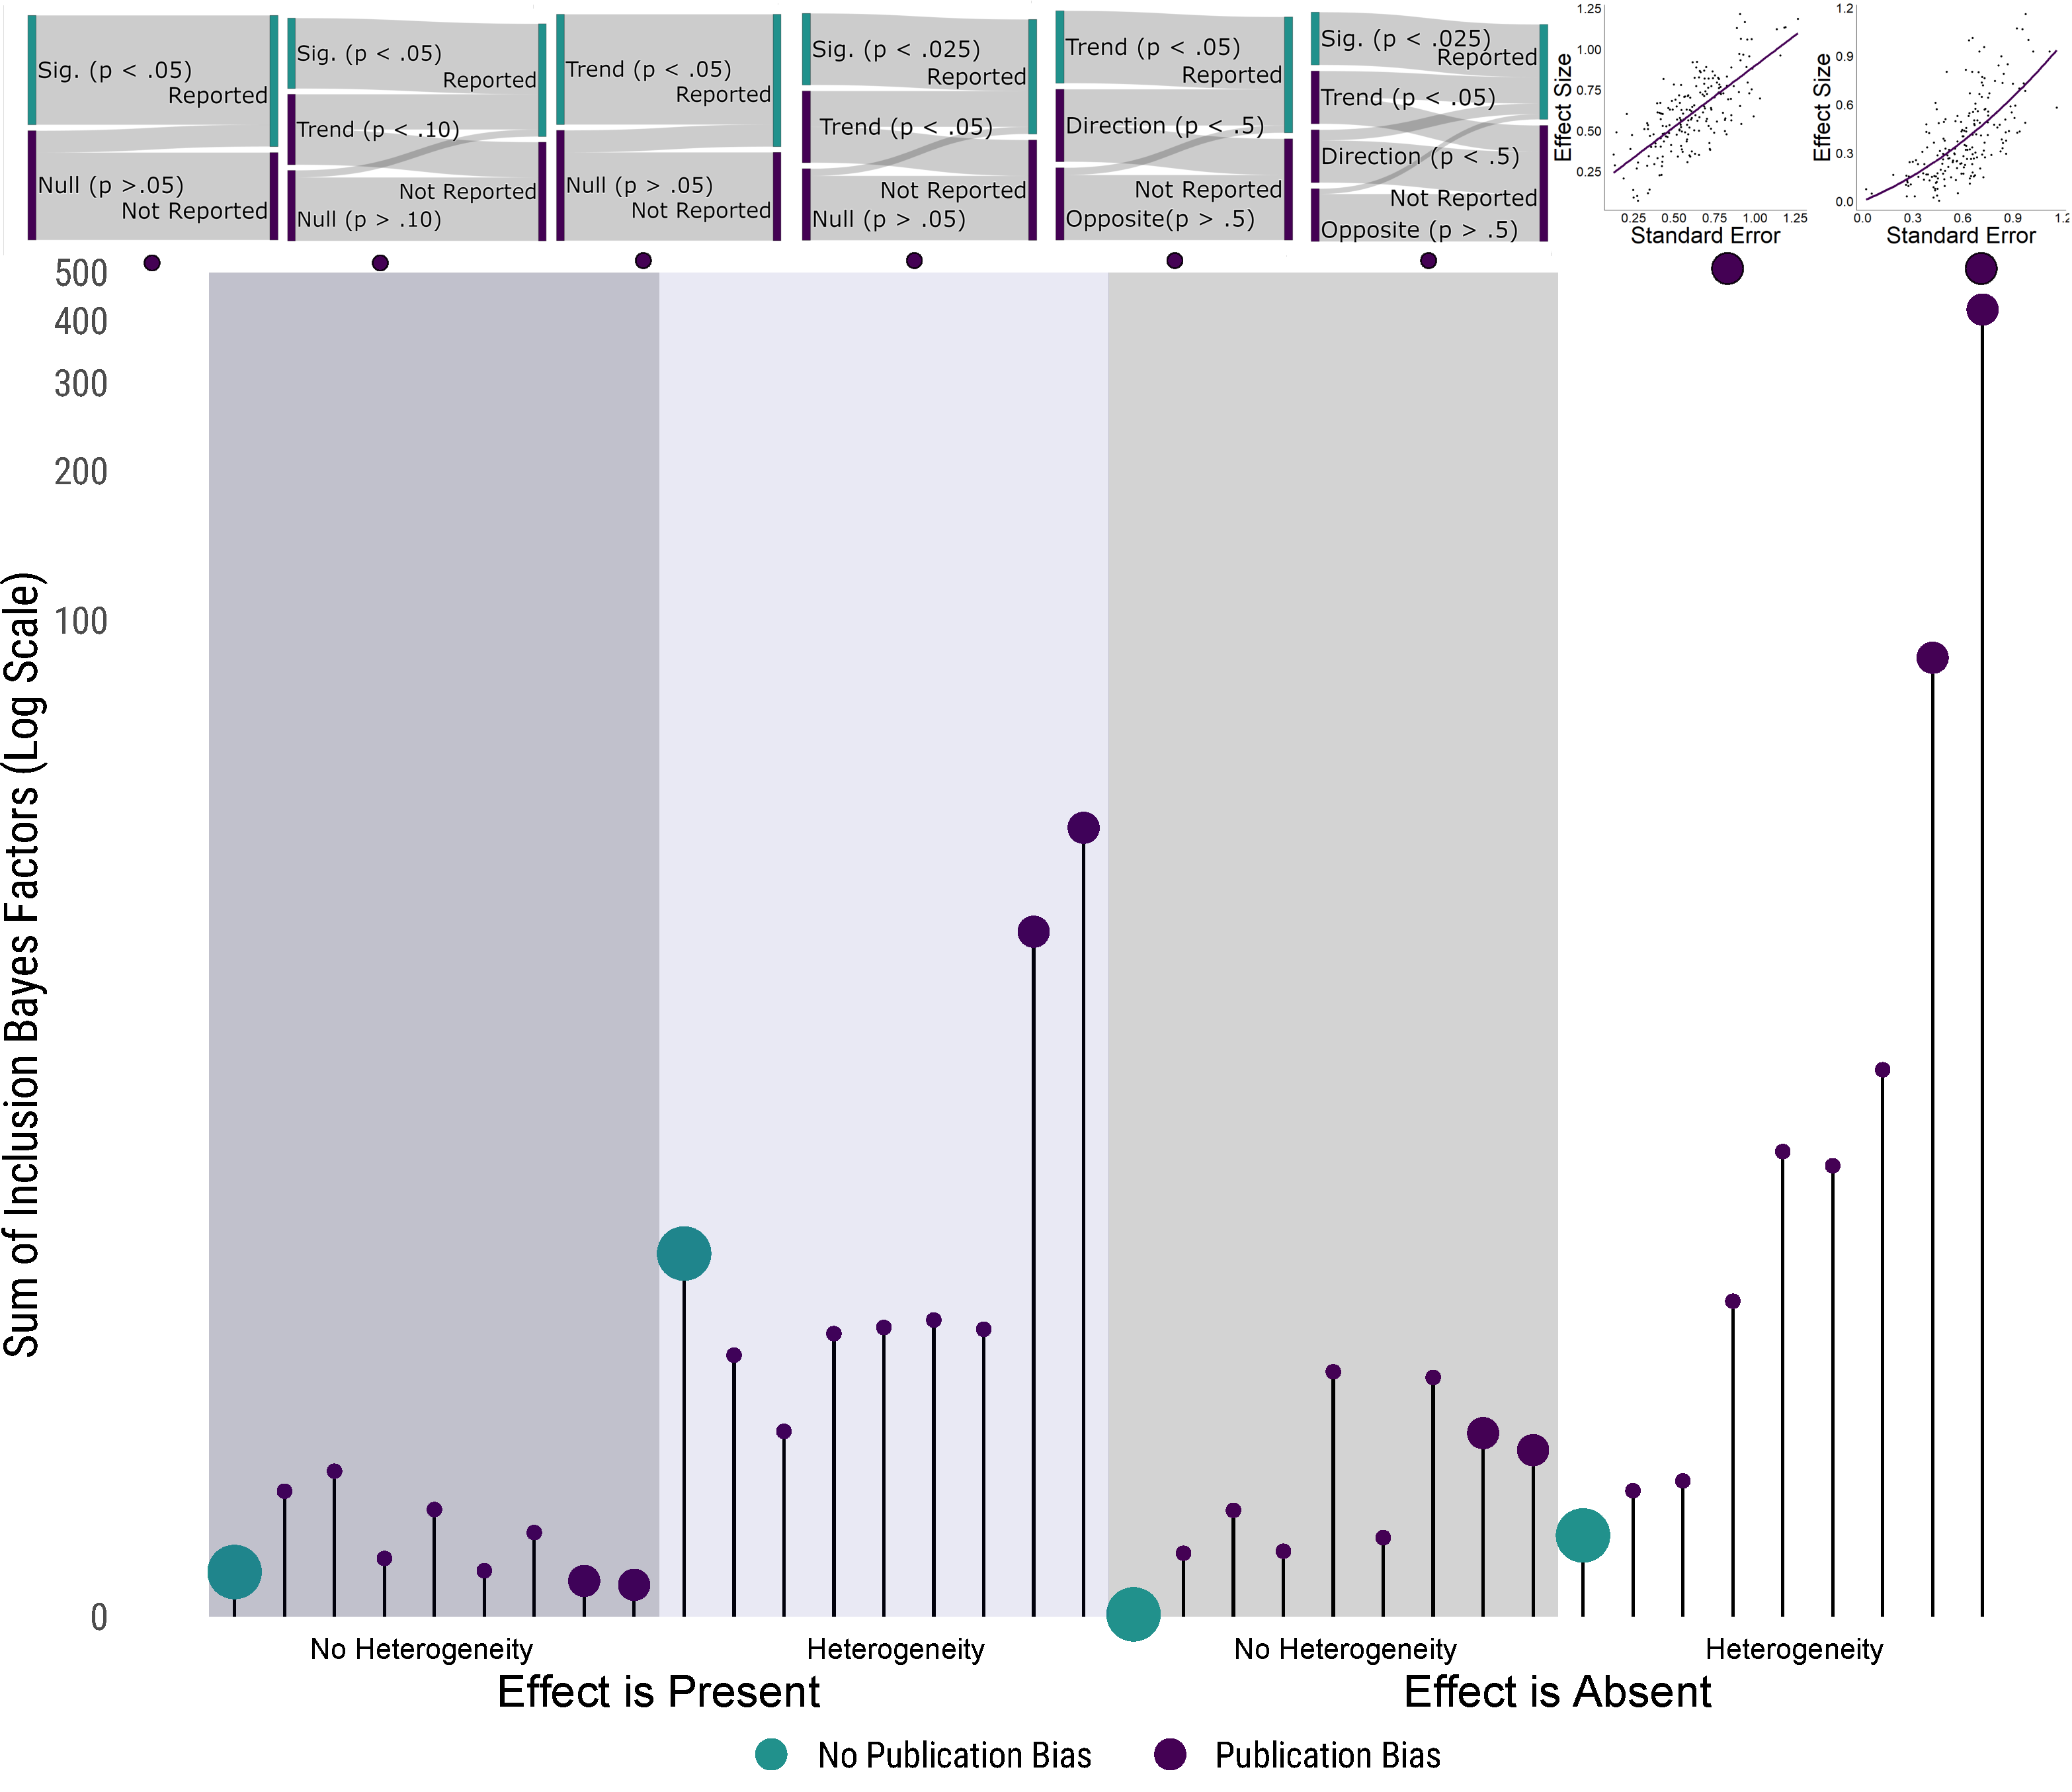
\includegraphics[scale=0.28]{../../figs/fig3.pdf}
    \setlength{\belowcaptionskip}{-2em}
    \caption*{\singlespacing \small Note. \normalfont Higher Inclusion Bayes Factors indicate better agreement with the data than the average of the ensemble. The green circles represent naïve fixed and random effects models that assume no publication bias. The purple circles represent six selection models and two regression models, each modeling publication bias in a different way. A figure illustrating each of the publication bias models is displayed below the lollipop plot, shown in the same left-to-right order they follow in the plot above. The size of each circle reflects the prior probability assigned to the model (\emph{p} = 0.125 for naïve models, \emph{p} = 0.031 for regression models, and \emph{p} = 0.01 for selection models). The naïve and publication bias models were fit testing four scenarios: (a) an effect is present, no heterogeneity, (b) an effect is present, heterogeneity is present, (c) an effect is absent, no heterogeneity, and (d) an effect is absent, heterogeneity is present. The PEESE model, presented on the far right in each scenario, dominated the other models when assuming an effect is absent and heterogeneity is present. To better illustrate the performance of each model in the ensemble, Inclusion Bayes Factors are shown on a log scale on the \emph{y}-axis.}
    \label{fig:fig3}
\end{figure}

\clearpage

\section{Discussion}

We re-evaluated the evidence in support of an external focus benefit for learning, performance, muscular efficiency, and the distance effect. Seven previous meta-analyses have relied on the results of naïve random effects models that assume zero reporting bias in the primary estimates. However, it has become clear that such an assumption may not be appropriate for motor learning research \autocite{mckay2022b,mckay2023}. Each of the previous seven meta-analyses concluded that an external focus is superior to an internal focus. Kim et al. (\citeyear{kim2017}) reported the benefits applied to balance learning, performance, and transfer. \textcite{makaruk2020} found the same for jump performance and \textcite{li2022} reported similar results for sprint performance. Grgic and colleagues reported external focus benefits for both muscular strength and endurance \autocite{grgic2021,grgic2022}. \textcite{nicklas2022} reported the advantage of an external focus over an internal focus applied to immediate performance in general. The most comprehensive of the meta-analyses, and the study whose data we reanalyzed, was conducted by \textcite{chua2021}. They estimated small to moderate benefits for each specific effect and concluded that no amount of publication bias could attenuate the observed effects to zero.

Our results differ from previous meta-anayses as reporting bias was unaccounted for in their primary estimates. This is a serious limitation of the previous external focus meta-analyses as simulation studies have clearly demonstrated that random-effects models result in large biases and high rates of false positives in the presence of publication-selection bias \autocite{bartos2023a,bom2019,stanley2017,stanley2022}, which have been further supported when random-effects are compared with preregistered multilab replications \autocite{kvarven2020}. We therefore explicitly modeled bias; and consequently, estimated trivially small effects in each analysis. Although \textcite{chua2021} concluded that no amount of publication bias could reduce the effects to the null, our models suggest the data favor the null hypothesis for each analysis. If the only type of reporting bias in the literature is one-sided selection at \emph{p} = 0.05, then Chua and colleagues' conclusions were justified. However, if there were other considerations, such as sample size, trends, and direction of point estimates, the assumptions of their model were violated. Our analysis suggests this is the case for the focus of attention literature. Thus, similar to previous simulation studies our findings illustrate that reporting bias can cause random effects models to produce even large effect estimates when the true model is null. The random effects estimates reported by \textcite{chua2021} ranged from small to large and our corrected estimates range from essentially nil to trivial at most.

Although we observed somewhat larger estimates among effects selected by \textcite{chua2021} than among alternative outcomes that could have been selected, the difference was small and easily attributable to chance. The stronger signal for selection came from censorship prior to appearing in the published sample. Thus, the average reader of this literature would not have been inoculated against bias by having access to the complete results of each article. The biasing influence of censorship would have already affected the sample of information readers could access.

These findings underscore uncertainty about external focus benefits. Adding to this uncertainty, we observed significant unexplained heterogeneity in effects. This heterogeneity could imply that focus of attention has a range of effects that depend on situational factors. If so, our results suggest that an internal focus may be superior to an external focus in nearly as many situations as the reverse. Alternatively, this heterogeneity may be due to methodological idiosyncrasies, unmodeled selection, or poor data curation at any level. As with censorship mechanisms, we have no way to know which potential sources of heterogeneity were at play.

Unfortunately, the present results add to a growing body of metascience questioning the extant support for the predictions in Wulf and Lewthwaite's (\citeyear{wulf2016}) OPTIMAL theory of motor learning \autocite[see][for a recent meta-analysis on the other two pillars in the theory]{mckay2023}. In addition to predicting external focus benefits for learning and performance, OPTIMAL theory also predicts beneficial effects for autonomy and enhanced expectancies via similar underlying mechanisms \autocite{wulf2016}. The primary corpus of evidence supporting motor learning benefits from autonomy is the self-controlled practice literature. Self-controlled practice involves asking learners to choose an aspect of their practice environment and the published literature suggests this will confer noticeable benefits to performance and learning \autocite[for a review see][]{stemarie2020}. However, like the external focus literature, the self-controlled practice research shows substantial evidence of reporting bias and more support for the null hypothesis \autocite{mckay2022b}. Approximately the same pattern emerges for the enhanced expectancies research \autocite{bacelar2022b}. Although the published literature appears to unequivocally demonstrate the predicted motor benefits of enhancing a learner's expectancy for success, accounting for reporting bias suggests uncertainty and heterogeneity \autocite{mckay2023}. Taken together, this meta-evidence suggests the underlying mechanism common to all three factors of the tripartite OPTIMAL theory may be censorship. The mechanisms forwarded in OPTIMAL theory are made no less valid by this conclusion; it is the evidence rather than the theory that has been impugned by this body of work.\footnotemark{}

\footnotetext{This conclusion also applies to other theories and perspectives (e.g., ecological dynamics) that have been forwarded based on the extant attentional focus literature to account for a supposed external focus advantage \autocite[e.g.,][]{davids2003,wulf2001,prinz1990,hommel2001,gottwald2023}.}

\subsection{Limitations}

By reanalyzing the dataset from \textcite{chua2021}, we inheritted the limitations of their original study, including restricting the literature search to studies published in English. Our results highlight the impact of reporting bias, which may be a systemic issue with contributions from authors, reviewers, editors, journals, institutions, and funders. By excluding articles not published in English, this dataset omits studies that have potentially been reported from outside the Western cultural milieu, where the impact of systemic pressures may be expressed differently. Further, because studies that have not been published were omitted, and these studies may or may not have been subjected to the scrutiny of peer-review and editorial discretion, this dataset does not represent a total account of all studies ever conducted on external focus of attention and the impact of systemic factors on reporting bias. Although the dataset is restricted to published studies that have been peer-reviewed, and \textcite{chua2021} thoroughly probed the risk of bias among those studies, such efforts are no guarantee on the accuracy of the underlying data \autocite[see][]{mckay-carter2023}. Caution is always warranted when interpreting the results of a retrospective meta-analysis of non-Registered Reports, especially without individual participant data.

Overall, the evidence in the review contains small sample sizes and small to moderate risk of bias according to Chua and colleagues (\citeyear{chua2021}). None of the studies were preregistered. There were 20 studies missing due to insufficient information to calculate effect sizes in the original data set and another four missing effects from our extraction of secondary outcomes. We excluded as many as four outliers based on leverage statistics whereas \textcite{chua2021} removed as many as 18 outliers using a different criteria. We recommend that, moving forward, researchers conducting meta-analyses in motor learning and related areas (e.g., psychology, neuroscience, sport and exercise science) adopt the use of leverage statistics as the default approach for identifying outliers \autocite[see][for discussions]{deeks2023,viechtbauer2010a}.

Lastly, we did not explore whether manipulation checks verified that the instructed attentional focus was adopted during performance. OPTIMAL theory predicts that when learners focus on their intended effect on the environment, they facilitate goal-action coupling, benefiting performance and learning. Our analysis only investigated whether instructions or feedback impacted performance. Perhaps a missing moderator in our analysis was the extent to which focus instructions were followed in each experiment. We chose not to explore this possibility because there are no validated manipulation checks.

\subsection{Recommendations and Conclusions}

The potential benefit of adopting an external focus of attention is among the most important contributions of academic motor learning research. It fits with numerous theoretical perspectives in the scientific literature and has been widely promoted in an array of applied settings, including sports, rehabilitation, and education. Our findings impugn the evidential basis for the superiority of an external focus of attention. However, rather than establishing nil or trivial benefits from focusing externally, uncertainty remains. The posteriors include interesting effects, there may be important moderators, and our estimates may have overcorrected for bias. We simply do not know if an external focus provides meaningful benefits to motor learning and performance or not.

Building knowledge about external focus effects can be accelerated by adoption of the Registered Report publication format \autocite{chambers2019}. Registered Reports prevent publication bias \autocite{scheel2021}, and when they include preregistration of analysis plans, they prevent \emph{p}-hacking \autocite{simmons2011} and HARKing \autocite{kerr1998} as well. Limited resources may prevent individual laboratories from collecting sufficient sample sizes for a well-powered Registered Report, so researchers are encouraged to collaborate extensively to achieve the sample sizes necessary to make progress.

\newpage

\subsection{Author contributions (CRediT Taxonomy)}

\noindent Conceptualization: BM, MJC\\
\noindent Data curation: BM, MJC\\
\noindent Formal analysis: BM\\
\noindent Funding acquisition: MJC\\
\noindent Investigation: BM, AEC, JS, CSDF, HH, KA, FCA, MJC\\
\noindent Methodology: BM, MJC\\
\noindent Project administration: BM, MJC\\
\noindent Software: BM, MJC\\
\noindent Supervision: MJC\\
\noindent Validation: BM, MJC\\
\noindent Visualization: BM, MJC\\
\noindent Writing -- original draft: BM, AEC, JS, CSDF, HH, KA, FCA, MJC\\
\noindent Writing -- review \& editing: BM, AEC, JS, CSDF, HH, KA, FCA, MJC

\subsection{Data availability statement}

\noindent The data and scripts can be accessed using either of the following links: \url{https://osf.io/vfmx2/} or \url{https://github.com/cartermaclab/proj_foa-optimal-theory}

\subsection{Declaration of interest statement}

\noindent All authors declare no conflicts of interest.

\subsection{Funding}

\noindent This work was supported by the Natural Sciences and Engineering Research Council (NSERC) of Canada (RGPIN-2018-05589; MJC) and McMaster University (MJC).


\nocitemeta{abdollahipour2008-meta,abdollahipour2020-meta,abdollahipour2017-meta,abdollahipour2016-meta,abdollahipour2014-meta,abdollahipour2015-meta,agar2016-meta,ahmad2013-meta,asadi2015-meta,ashraf2017-meta,beck2017-meta,beck2018can,becker2013-meta,brocken2016-meta,chiviacowsky2013-meta,chiviacowsky2010-meta,chow2014-meta,christina2014-meta,coker2016-meta,coker2018-meta,teixeira2017-meta,de2017-meta,diekfuss2018-meta,ducharme2015-meta,ducharme2016-meta,duke2011-meta,durham2014-meta,emanuel2008-meta,fasoli2002-meta,flores2015-meta,freudenheim2010-meta,gredin2016-meta,greig2014-meta,hadler2014-meta,halperin2017-meta,halperin2016-meta,halperin2016b-meta,hebert2017-meta,hill2017-meta,hosseiny2014c-meta,huang2014-meta,ille2013-meta,jackson2011-meta,jazaeri2018-meta,kal2013-meta,kalkhoran2014-meta,kearney2015-meta,kim2017-meta,klostermann2014-meta,koufou2013-meta,kuhn2018-meta,kuhn2017-meta,land2014-meta,landers2016-meta,landers2005-meta,laufer2007-meta,lawrence2011-meta,lisman2013-meta,lohse2014-meta,lohse2011-meta,lohse2012-meta,lohse2010-meta,lohse2011b-meta,makaruk2012-meta,makaruk2015-meta,makaruk2013-meta,marchant2019-meta,marchant2009-meta,marchant2017-meta,marchant2009b-meta,marchant2018-meta,maurer2013-meta,mckay2012-meta,mcnevin2003-meta,mcnevin2013-meta,mornell2019-meta,mullen2012-meta,nadzalan2015-meta,neumann2013-meta,oki2018-meta,palmer2017-meta,parr2009-meta,pelleck2017-meta,perkins2003-meta,perreault2015-meta,polskaia2015-meta,porter2011-meta,porter2013-meta,porter2012-meta,porter2010-meta,porter2013b-meta,porter2015-meta,querfurth2016-meta,raisbeck2019-meta,richer2017-meta,rossettini2017-meta,saemi2016-meta,saemi2013-meta,samsudin2017-meta,schucker2013-meta,schucker2016-meta,schucker2009-meta,schucker2015-meta,schucker2016b-meta,schutts2017-meta,shafizadeh2013-meta,shafizadeh2013b-meta,shea1999-meta,shea1999-meta,sherwood2014-meta,stambaugh2017-meta,stoate2011-meta,tse2019-meta,tse2017-meta,tsetseli2016-meta,tsetseli2018-meta,uehara2008-meta,vance2004-meta,welling2016-meta,winkelman2017-meta,wu2012-meta,wulf2008-meta,wulf2010-meta,wulf2009-meta,wulf2010b-meta,wulf1998-meta,wulf2009b-meta,wulf1999-meta,wulf2002-meta,wulf2001-meta,wulf2007-meta,wulf2007b-meta,wulf2003-meta,wulf2003b-meta,wulf2007c-meta,yogev2017-meta,zachry2005-meta,zarghami2012-meta,zentgraf2009-meta,ziv2015-meta,ziv2013-meta}


\defbibnote{asterisk}{\indent References marked with an asterisk indicate articles included in the meta-analyses.}
\printbibliography[title=References,prenote=asterisk]
\renewcommand{\printbibliography}{}
%\printbibliography

\end{document}
